\documentclass[xcolor=dvipsnames]{beamer}
\usepackage[latin1]{inputenc}
\usepackage{graphicx}
\usepackage{verbatim}
\usepackage{amsmath}
\usepackage{amssymb}
\usepackage{float}
\usepackage{hyperref}
\usepackage{listings}
\usepackage{authblk}
\usepackage{gensymb}
\usepackage{subcaption}
\usepackage[]{algorithm2e}
\usepackage{color}

\usecolortheme[named=Brown]{structure}
\usetheme{Malmoe}


\definecolor{dkgreen}{rgb}{0,0.6,0}
\definecolor{gray}{rgb}{0.5,0.5,0.5}
\definecolor{mauve}{rgb}{0.58,0,0.82}

\lstset{frame=tb,
  language=Java,
  aboveskip=3mm,
  belowskip=3mm,
  showstringspaces=false,
  columns=flexible,
  basicstyle={\small\ttfamily},
  numbers=none,
  numberstyle=\tiny\color{gray},
  keywordstyle=\color{blue},
  commentstyle=\color{dkgreen},
  stringstyle=\color{mauve},
  breaklines=true,
  breakatwhitespace=true
  tabsize=3
}

\title{Bug Fixing in SMC}
\author{Phillip Wilt}\institute{University of Washington}

\begin{document}

\begin{frame}

\maketitle

\end{frame}

\begin{frame}

\centerline{Let's all smash bugs together!}

\begin{figure}[H]
    \centering
        
\includegraphics[width=1\textwidth]{bug}
\end{figure}

\end{frame}

\begin{frame}

\frametitle{Oh nos! What is this crazy error?}

sage: arrow([1,2,1],[2,1])

\vspace{3mm}

TypeError: unsupported operand parent(s) for '-': 'Vector space of dimension 2 over Real Double Field' and 'Vector space of dimension 3 over Real Double Field'

\end{frame}

\begin{frame}

\centerline{Stack traces and digging around in code and...}

\begin{figure}[H]
    \centering
        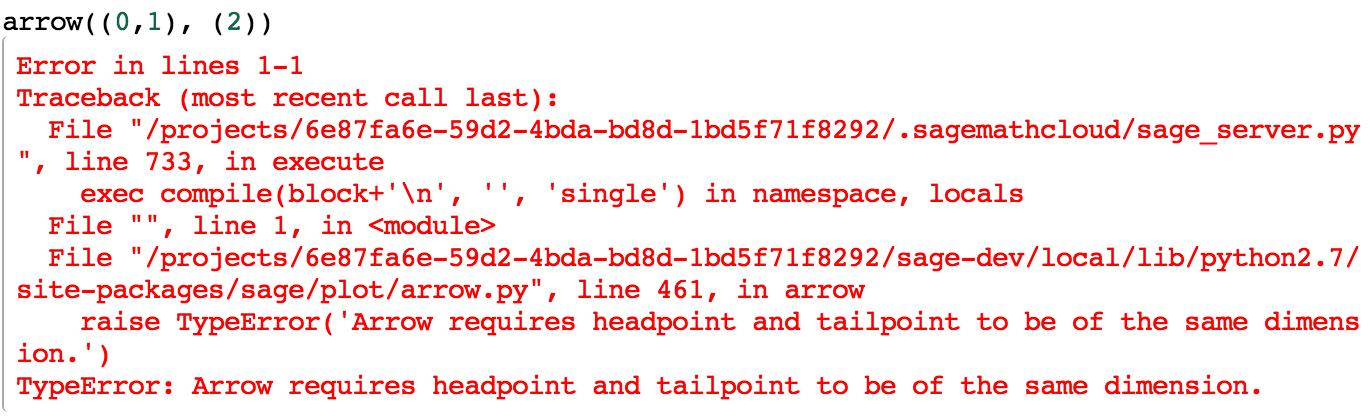
\includegraphics[width=.80\textwidth]{arrowbug}
\end{figure}

\centerline{Viola! Better error message!}

\end{frame}

\begin{frame}

\frametitle{Why the heck can't we do this?}

sage: arrow([1],[1])

\vspace{3mm}

ArithmeticError: Cross product only defined for vectors of length three or seven, not (3 and 1)

\end{frame}

\begin{frame}

\frametitle{Arrow Plotting!}

\begin{figure}[H]
    \centering
        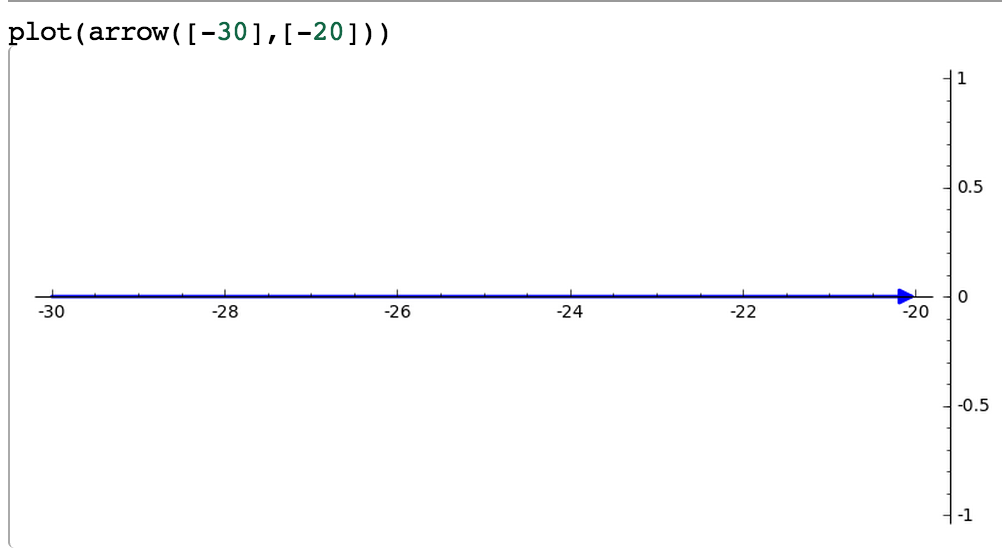
\includegraphics[width=.80\textwidth]{arrow}
\end{figure}

\centerline{Doesn't look like much, but Sage didn't do this before!}

\end{frame}

\begin{frame}

\frametitle{Who wants to help?}

\begin{figure}[H]
    \centering
        
\includegraphics[width=.85\textwidth]{handsup}
\end{figure}

\centerline{You do! But what do you need?}

\begin{itemize}
  \item git
  \item Web Browser (Chrome is best)
  \item {\Large The knowledge you already have from this class!}
\end{itemize}

\end{frame}

\begin{frame}

\frametitle{But don't I need a complex dev environment?}

\begin{figure}[H]
    \centering
        
\includegraphics[width=1\textwidth]{zoolander}
\end{figure}

How many software packages allow you to develop the software IN THE SOFTWARE?

\end{frame}

\begin{frame}

\frametitle{How Awesome is SageMathCloud?}

\begin{figure}[H]
    \centering
        
\includegraphics[width=.55\textwidth]{awesomesauce}
\end{figure}

\centerline{Freakin' AWESOME that's how awesome!}

%\vspace{3mm}

%Sage competes with large commercial math software like Maple, Mathematica, Matlab... but Sage is WAY more kewl.

\end{frame}

\begin{frame}

\frametitle{So who wants to help?}

\begin{figure}[H]
    \centering
        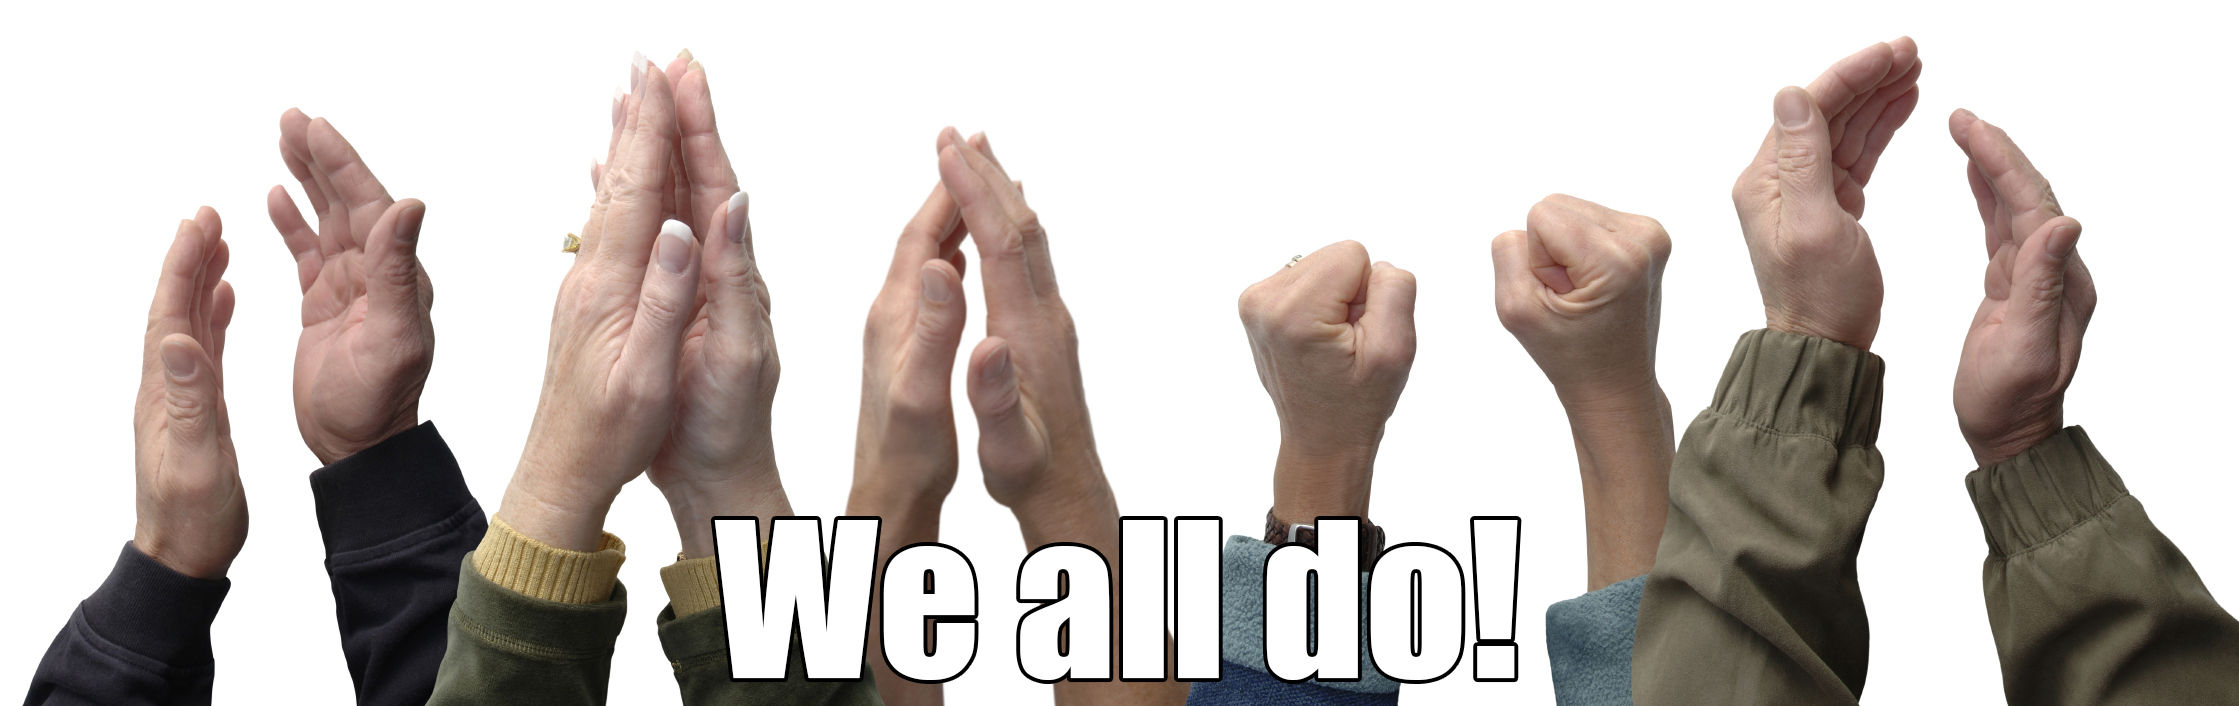
\includegraphics[width=1\textwidth]{clapping}
\end{figure}

\end{frame}

\begin{frame}

\frametitle{Look at these beginner bugs!}

\begin{figure}[H]
    \centering
        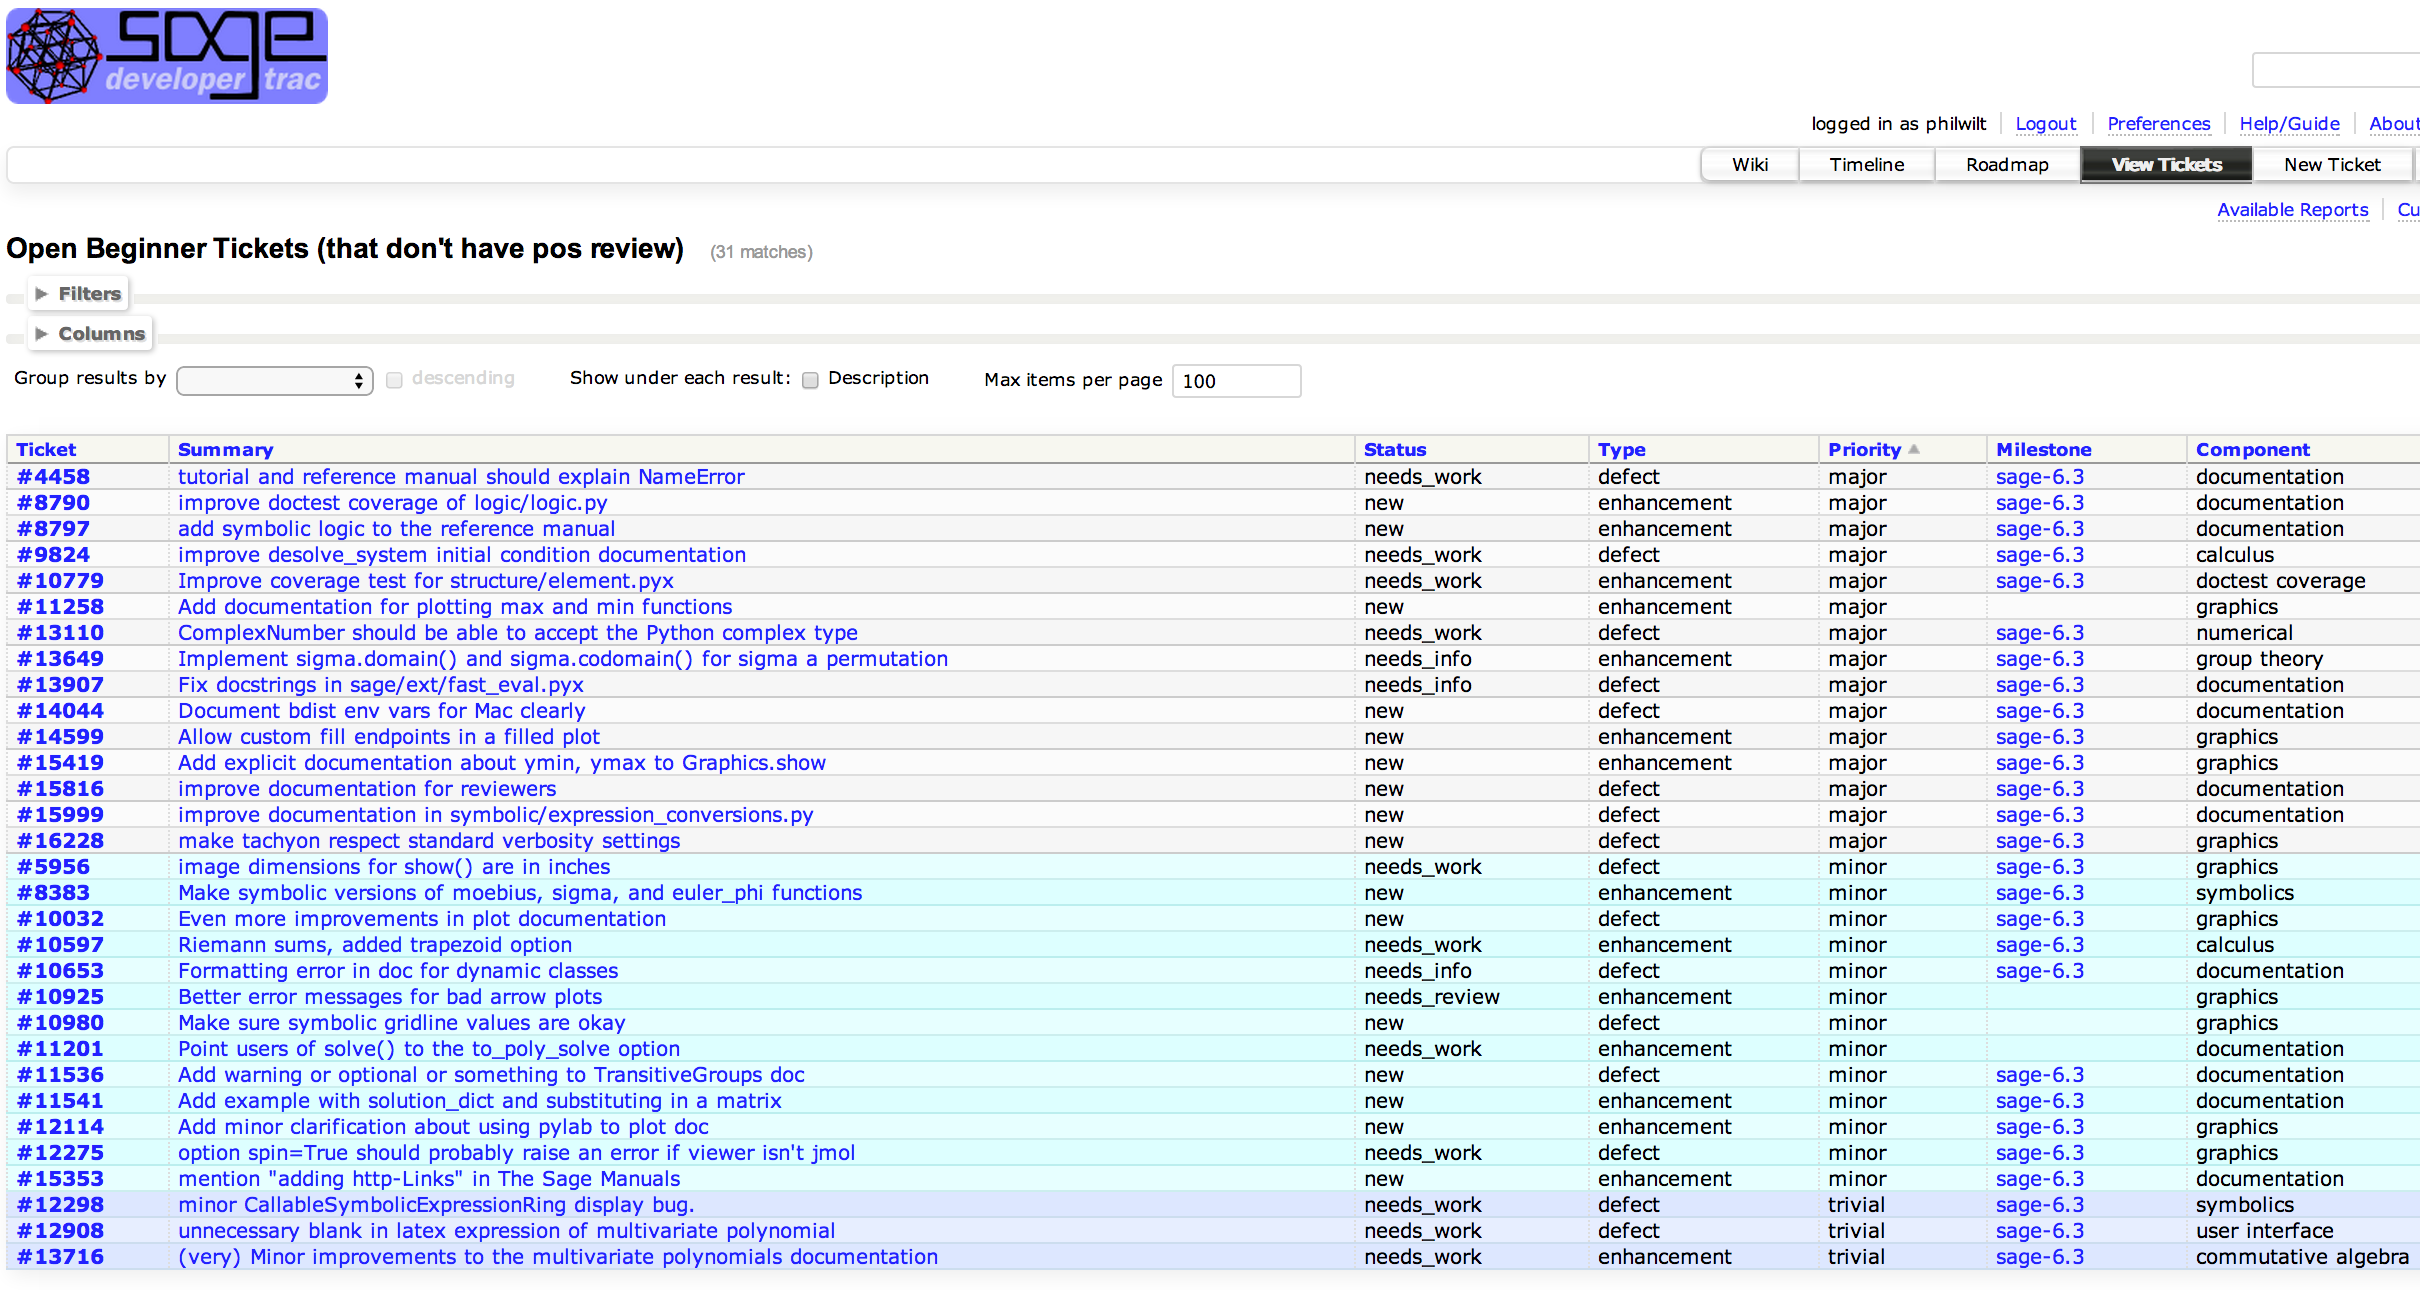
\includegraphics[width=1\textwidth]{beginbugs}
\end{figure}

\end{frame}

\begin{frame}

\centerline{Be the developmer you want to see in SMC!}

\begin{figure}[H]
    \centering
        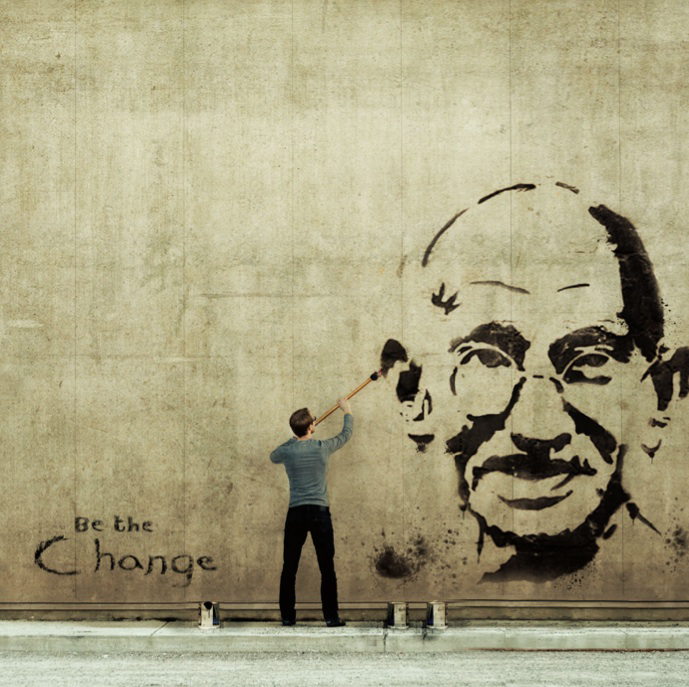
\includegraphics[width=.60\textwidth]{bethechange}
\end{figure}

\end{frame}


\end{document}
%sagemathcloud={"zoom_width":90}